\chapter{Lecture-2 May, 20, 2021}

\section{Why need non-linear activation function for hidden layer?}

\noindent{\color{red} \rule{\linewidth}{0.5mm}}
% ====================================================================================
\section{Why threshold is essentially important?}
\noindent{\color{red} \rule{\linewidth}{0.5mm}}
% ====================================================================================
\section{Learning in Artificial Neural Network, ANN}
Recall that there are 3 types of learning for neural networks:
\begin{itemize}
    \item Supervised
    \item Unsupervised
    \item Reinforcement
\end{itemize}
\textbf{Perceptron} is one of the supervised learning method . The activation function is hard limiter (+/- 1) function. The activation function is nonlinear and perceptron is used for classification.

\subsection{Single Neuron Perceptron}
Consider a single neuron with 2 inputs, the model can be written as 
\begin{equation}
y =hardlimit( \mathbb{W}\mathbb{X}+\theta)
 =hl(w_1x_1+w_2x_2+\theta)
\end{equation}
Where we use the second representation of the hard limiter function:
\begin{equation}
y = hl(x) = \left\{ {\begin{array}{*{20}{c}}
{1{\textrm{ if }}x \ge 0}\\
{ 0 {\textrm{ if }}x < 0}
\end{array}} \right.
\end{equation}
The "decision boundary" is determined by
\begin{equation}
 w_1x_1+w_2x_2+\theta = 0   
\end{equation}

\begin{center}
\begin{tikzpicture}
\Vertex[x=0,RGB,color={190,174,212},label=\(x_0\)]{A} 
\Vertex[x=2,label=\(x_1\)]{B}
\Vertex[x=4,label=\(x_2\)]{C}


\Vertex[x=2,y=-2,label=Neuron,size = 1]{E}
\Vertex[x=2,y=-4, label=y]{F}

\Edge[bend=-10,Direct=true,label=$\theta$](A)(E)
\Edge[bend=-5,Direct=true,label=w1](B)(E)
\Edge[bend=5,Direct=true,label=w2](C)(E)

\Edge[bend=0,Direct=true](E)(F)
\end{tikzpicture}
\end{center}
\subsection*{Exmp: Build a perceptron to simulate an AND gate}
The question is basically asking to find the decision boundary of a AND gate, there are Inf. many possible solutions for this question, and we are going to find one via supervised learning.
\begin{center}
\begin{tabular}{|l|l|l|l|l}
\hline
            & \textbf{X1} & \textbf{X2} & \textbf{y} \\ \hline
\textbf{P1} & 0           & 0           & 0          \\ \cline{1-4}
\textbf{P2} & 1           & 0           & 0          \\ \cline{1-4}
\textbf{P3} & 0           & 1           & 0          \\\cline{1-4}
\textbf{P4} & 1           & 1           & 1          \\ \hline
\end{tabular}
\end{center}

\begin{center}
    \begin{tikzpicture}
\begin{axis}[
    axis lines=middle,
    xmin=-0.5, xmax=2,
    ymin=-0.5, ymax=2,
    xlabel={$x1$},
    ylabel={$x2$}],
    ]
\addplot [smooth,blue,name path=A,no marks] {-x+1.5}; % actual curve
\addplot [draw=none,name path=B, no marks] {2.3};     % “fictional” curve
\addplot [green!40,opacity=0.5] fill between[of=A and B,soft clip={domain=-4:4}]; % filling
\addplot [smooth, blue, name path=C, no marks,domain=0:0.8] {x};     % “fictional” curve
\addplot[color=red,only marks,] coordinates {(0,0)(1,0)(0,1)};
\addplot[color=red, only marks, mark=star]coordinates{(1,1)};
\addplot[black](1.2,1.6) circle (0pt) node[anchor=west] {y=1 region};
\addplot[black](0,0) circle (3pt) node[anchor=south] {P1};
\addplot[black](1,0) circle (3pt) node[anchor=south] {P2};
\addplot[black](0,1) circle (3pt) node[anchor=west] {P3};
\addplot[black](1,1) circle (3pt) node[anchor=west] {P4};

\end{axis}
\end{tikzpicture}
\end{center}
\\
\\By observation, one can pick the decision boundary passing through (1.5, 0) and (0, 1.5), so that this decision boundary can separate dot from star.
\\
\\
To find the $w_1$, and $w_2$ and $\theta$ for this decision boundary:
\textcolor{red}{Normally, we choose $\mathbb{W}$ vector perpendicular to the D.B, and toward the y = 1 region.} \textcolor{brown}{So, what should we do in general case if \mathbb{W} is a M by N+1 matrix???}
\\
\\
From graph, we can tell that $\mathbb{W}$ is in the 45 degree angle (perpendicular to D.B. and toward to y = 1 region). Let $\mathbb{W} = [1,1]$, then we have the D.B. as: 
\begin{equation}
 x_1+x_2+\theta = 0   
\end{equation}
We also know that the D.B. passing point (1.5, 0):
\begin{equation}
 1.5 + 0 +\theta = 0   
\end{equation}
Finally, we get $\theta = -1.5$, and the D.B can be written as: 
\begin{equation}
 x_1+x_2-1.5 = 0   
\end{equation}
\subsection{Multiple Neurons Perceptron}
The model for multiple neurons perceptron with N inputs, M outputs, and M neurons, its D.B. of the jth neuron can be written as:
\begin{equation}
 \mathbb{W}_j\mathbb{X}+\theta_j = 0   
\end{equation}
In general, we have 
\begin{equation}
 \mathbb{W}_{(MXN)}\mathbb{X}_{(NX1)}+\theta_{(MX1)} = 0   
\end{equation}
Note that for a single neuron, y = 1 or 0, the perceptron provides two possible classes; while for M neurons, we have $y = 2^{M}$ possible classes;


\noindent{\color{red} \rule{\linewidth}{0.5mm}}
% ====================================================================================
\section{Perceptron Learning Rules}

\[\mathbb{W}_{MXN}^{new} = {\mathbb{W}^{old}} + (\mathbb{t} - \mathbb{y}){\mathbb{X}^T} = {\mathbb{W}^{old}} + {\mathbb{e}_{MX1}}\mathbb{X}_{1XN}^T\]

\[\mathbb{\theta}_{MX1}^{new} = {\mathbb{\theta}^{old}} + {\mathbb{e}_{MX1}}\]

If combine the weight and threshold together, we can get:
\[\mathbb{W}_{MX(N+1)}^{new} = {\mathbb{W}^{old}} + (\mathbb{t} - \mathbb{y}){\mathbb{X}^T} = {\mathbb{W}^{old}} + {\mathbb{e}_{MX1}}\mathbb{X}_{1X(N+1)}^{*T}\]
Where $\mathbb{X}^{*}$ is the argument-ed input vector, and can be written as below:
\[\left[ {\begin{array}{*{20}{c}}
{{x_0} \equiv 1}\\
{{x_1}}\\
 \vdots \\
{{x_N}}
\end{array}} \right]\]

\subsection*{Exmp}
Design a  single neural perceptron by learning for a 3 input system, where:
\[\begin{array}{*{20}{c}}
{\mathbb{X}_1 = \left[ {\begin{array}{*{20}{c}}
{{1}}\\
{{-1}}\\
{{-1}}
\end{array}} \right]}&,&{t_1 = 0}
\end{array}\]
\[\begin{array}{*{20}{c}}
{\mathbb{X}_2 = \left[ {\begin{array}{*{20}{c}}
{{1}}\\
{{1}}\\
{{-1}}
\end{array}} \right]}&,&{t_2 = 1}
\end{array}\]
\begin{center}

\centering
\begin{tabular}{llllll}
\multicolumn{1}{c}{}
& X_0 &X_1  &X_2  &X_3  &t   \\ \hline
P1 & 1 &1  & -1 & -1 &0   \\
 P2& 1 & 1 & 1 & -1 & 1 
\end{tabular}
\end{center}

\begin{center}
\begin{tikzpicture}
\Vertex[x=0,RGB,color={190,174,212},label=\(x_0\)]{A} 
\Vertex[x=2,label=\(x_1\)]{B}
\Vertex[x=4,label=\(x_2\)]{C}
\Vertex[x=6,label=\(x_3\)]{D}
\Vertex[x=8,label=\(x_4\)]{G}


\Vertex[x=4,y=-2,label=Neuron,size = 1]{E}
\Vertex[x=4,y=-4, label=y]{F}

\Edge[bend=-10,Direct=true,color=red,label=$\theta$](A)(E)
\Edge[bend=-5,Direct=true,label=w1](B)(E)
\Edge[bend=5,Direct=true,label=w2](C)(E)
\Edge[bend=5,Direct=true,label=w3](D)(E)
\Edge[bend=5,Direct=true,label=w4](G)(E)
\Edge[bend=0,Direct=true](E)(F)
\end{tikzpicture}
\end{center}
\\
Solution: We will randomly choose:
\[\begin{array}{*{20}{c}}
{\mathbb{W} = \left[ {\begin{array}{*{20}{c}}
{{0.5}}\\
{{-1}}\\
{{-0.5}}
\end{array}} \right]^{T}}&,&{\theta = 0.5}
\end{array}\]
\textcolor{red}{As a rule of thumb, $\mathbb{W}$ should between -1 and +1.} One can re-write $\mathbb{W}$ in argumented format:
\[{\mathbb{W}_0=\left[ {\begin{array}{*{20}{c}}
{0.5}\\
{0.5}\\
{ - 1}\\
{ - 0.5}
\end{array}} \right]^{T}\]

For $\mathbb{X}_1$:
\[y_1=hl(\mathbb{W}^{0}\mathbb{X}_1^{*})=1\]
\[e = t-y = 0-1 = -1\]
\[\mathbb{W}^1 = \mathbb{W}^0-\mathbb{X}_{1}^{*}=\left[ {\begin{array}{*{20}{c}}
{-0.5}\\
{-0.5}\\
{0}\\
{0.5}
\end{array}} \right]^{T}
\]

For $\mathbb{X}_2$:
\[y_2=hl(\mathbb{W}^{1}\mathbb{X}_2^{*})=0 \ne {t_2}\]
\[e = t-y = 1-0 = 1\]
\[\mathbb{W}^2 = \mathbb{W}^1+\mathbb{X}_{2}^{*}=\left[ {\begin{array}{*{20}{c}}
{0.5}\\
{0.5}\\
{1}\\
{-0.5}
\end{array}} \right]^{T}
\]

For $\mathbb{X}_1$ (the 3rd iteration):
\[y_1=hl(\mathbb{W}^{2}\mathbb{X}_1^{*})=1 \ne {t_1}\]
\[e = t-y = 0-1 = -1\]
\[\mathbb{W}^3 = \mathbb{W}^2+\mathbb{X}_{1}^{*}=\left[ {\begin{array}{*{20}{c}}
{-0.5}\\
{-0.5}\\
{2}\\
{0.5}
\end{array}} \right]^{T}
\]
For $\mathbb{X}_2$ (the 4th iteration), $e=0$, requires no learning:
\[y_2=hl(\mathbb{W}^{3}\mathbb{X}_2^{*})=1 = {t_2}\]
\[e = t-y = 1-1 = 0\]
For $\mathbb{X}_1$ (the 5th iteration), $e=0$, requires no learning:
\[y_1=hl(\mathbb{W}^{3}\mathbb{X}_1^{*})=0 = {t_1}\]
\[e = t-y = 0-0 = 0\]
We found one possible solution for this preceptron is: 
\[
\pushQED{\qed} 
\mathbb{W}^3 = \left[ {\begin{array}{*{20}{c}}
{-0.5}\\
{-0.5}\\
{2}\\
{0.5}
\end{array}} \right]^{T}\qedhere
\]

